\documentclass[12pt]{article}
\setlength{\textwidth}{17cm}
\setlength{\textheight}{24cm}
\setlength{\topmargin}{-2cm}
\setlength{\footskip}{1cm}
\setlength{\evensidemargin}{0cm}
\setlength{\oddsidemargin}{0cm}
\setlength{\parindent}{0cm}

\usepackage{allrunes}
\usepackage{amsmath}
\usepackage[magyar]{babel}
\usepackage[T1]{fontenc}
\usepackage[utf8]{inputenc}
\usepackage{fixltx2e}
\usepackage{multirow}

\usepackage[hyphens]{url}
\usepackage[unicode,colorlinks=true,breaklinks]{hyperref}
%\usepackage[dvips]{hyperref}
%should display links, but it does not work with \H accent
%and formulas in section titles

\hypersetup{colorlinks,linkcolor=blue,urlcolor=magenta,citecolor=magenta}
%Breaks long url`s in text, while keeping it one link:

\usepackage{amsfonts}
\usepackage{amsthm}
\usepackage{amssymb}


\theoremstyle{plain}
\usepackage{graphicx}

%\usepackage{gensymb}
\usepackage{float}

% For bra-ket notation
\usepackage{braket}

%% New commands
\newcommand{\dd}{\textrm{d}}

%% Pauli matrices
\newcommand{\sigx}{\sigma_x}
\newcommand{\sigy}{\sigma_y}
\newcommand{\sigz}{\sigma_z}

\newcommand{\paulix}{
    \left( \begin{array}{cc}
        0 & 1 \\
        1 & 0
    \end{array}
    \right)
}

\newcommand{\pauliy}{
    \left( \begin{array}{cc}
        0 & -i \\
        i & 0
    \end{array}
    \right)
}

\newcommand{\pauliz}{
    \left( \begin{array}{cc}
        1 & 0 \\
        0 & -1
    \end{array}
    \right)
}


\begin{document}
\title{10. tétel}
\author{Horváth Benedek}

\maketitle


\newpage
\begin{abstract}
    AD és DA konverterek – Digitális-analóg konverzió, AD-konverzió szukcesszív approximációval. A kvantálási zaj és a mintavételi törvény. Digitális jelek tömörítési módszerei: delta-moduláció és delta-szigma moduláció. Digitális számábrázolás és műveletvégzés.
\end{abstract}

\section{Bevezetés}

A számítógépes rendszerek önmagukban csak számokat tudnak értelmezni és előállítani, a bemenő- és kimenőmennyiségeik mértékegység nélküli digitális értékek. A mérhető fizikai mennyiségek azonban túlnyomórészt folytonosak, és a mérőeszközök jelentős része analóg jelet ad ki magából. Ezért mielőtt bármilyen digitális jelfeldolgozási eljárást hajtanánk végre, a fizikai valóság releváns mennyiségeit szükségszerűen át kell alakítani a digitális rendszerek által értelmezhető számokká úgy, hogy a számok az eredeti mennyiségeket hűen tükrözzék. A másik oldalról pedig, a számítógép vezérelheti a külvilágot (mérőberendezést), jellemzően egy feszültségjellel. Ilyenkor tehát a digitális műveletek eredményeit kell valamilyen arányos módon visszaalakítani valódi fizikai mennyiséggé. Összességében tehát a digitális-analóg és az analóg-digitális irányú átalakítás egyaránt gyakori a mindennapokban. A legkézenfekvőbb, mindkét irányú konverziót tartalmazó hétköznapi példa a számítógépes hangrögzítés, tárolás, feldolgozás, illetve hangszórón történő lejátszás. Ezekre a feladatokra dedikált áramköri egységek, az analóg-digitális (analog digital converter, ADC) és digitális-analóg (digital analog converter, DAC) átalakítók szolgálnak. Az eszközök egyszerű vázlata \aref{fig:konverter_vazlat}. ábrán látható. 


\begin{figure}[H]
	\centering
	\begin{minipage}{0.47\textwidth}
		\centering
		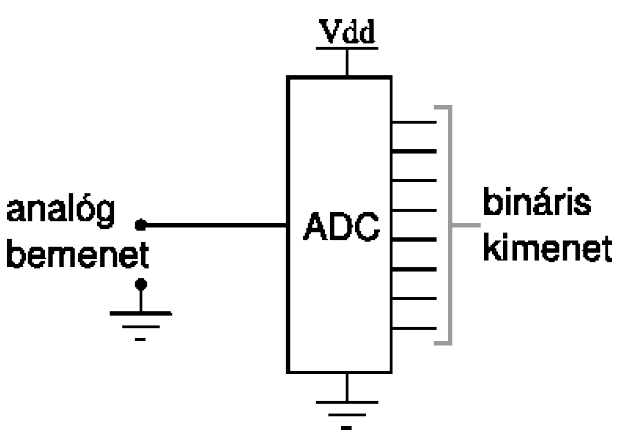
\includegraphics[width=1.0\textwidth]{./media/ADC_sketch.png}
	\end{minipage}\hfill
	\begin{minipage}{0.53\textwidth}
		\centering
		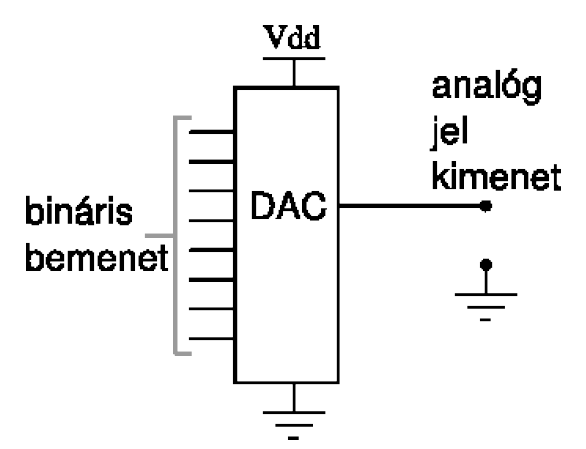
\includegraphics[width=0.85\textwidth]{./media/DAC_sketch.png}
	\end{minipage}
	\caption{Analóg-digitál (balra) és digitál-analóg (jobbra) konverter általános vázlata.}
	\label{fig:konverter_vazlat}
\end{figure}



\section{Digitális-analóg konverterek}

A digitális-analóg átalakítók (D/A konverterek) digitális jelek folytonossá alakítására használatosak. A D/A átalakítónak mind a bementi értéke, mind a kimeneti értéke az értékkészletében kvantált\footnote{Meg kell jegyezni, hogy ez az analóg oldalon természetesen csak elvileg igaz; a kimeneten fizikailag ténylegesen megjelenő feszültségérték időben folytonos. Nagy kvantumlépcső vagy alacsony mintavételi frekvencia esetén a kimeneti jelalak erősen torzított lesz az eredetihez képest, a felharmonikus tartalma igen magassá válik. Ennek jelentőségéről később ejtünk szót.}. Az alábbiakban két egyszerű elektronikai megvalósítását nézzük meg a digitális-analóg átalakítóknak.


\subsection{Bináris súlyozású DAC}

lkj


\begin{figure}
	\centering
	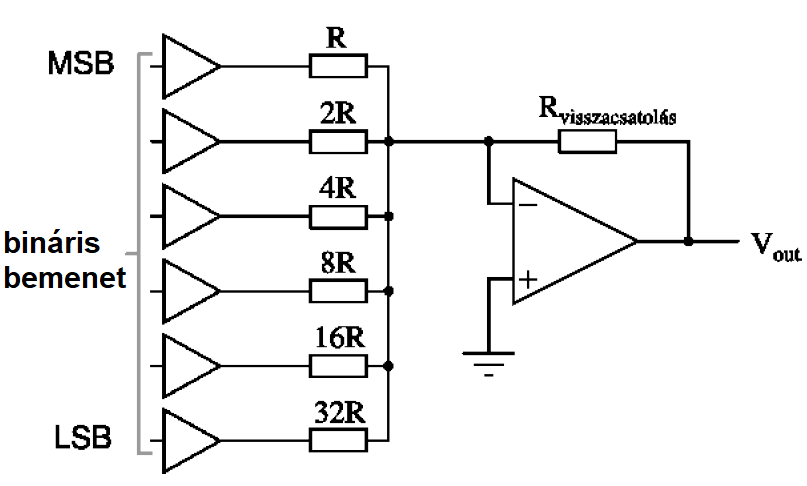
\includegraphics[width=0.7\linewidth]{media/DAC_binaris}
	\caption{6 bites bináris súlyozású digitális-analóg konverter áramköri vázlata.}
	\label{fig:dacbinaris}
\end{figure}


\subsection{R/2R létra}

fds





\section{Analóg-digitális konverterek}

Az analóg-digitális átalakítók a bemenetükre kapcsolt folytonos, analóg jelet egy órajel-generátor által meghatározott mintavételezési frekvencia szerint bináris számértékekké alakítják. Az áramkör kimenetén a jel feszültségszintjének digitális reprezentációja jelenik meg. Az A/D átalakítók általában a gyártó által előre meghatározott feszültségtartomány digitalizálására képesek, így a jel feszültségszintjét megfelelő analóg áramkörrel kell illeszteni az A/D konverter bemenetéhez. Az esetek többségében unipoláris A/D konvertereket alkalmaznak, amelyeknél a jeltartomány egyik széle általában a nulla, a méréshatár szélét végértéknek (Full Scale, FS) jelölik. A bipoláris pozitív-negatív átalakítók általában valamilyen szinteltolást alkalmaznak a bemeneten: a mérhető jeltartomány így közrefogja a nulla értéket, és általában szimmetrikus (FSR, Full Scale Range). Az átalakítók általában lineáris karakterisztikájúak, azaz a digitálisan megkülönböztetett szintek között egyenlő lépésközök vannak a bemenő analóg feszültségben. Egy ADC felbontóképességének azt az analóg jelváltozás nevezzük, ahol a kimenet vált, azaz ahol a változás megkülönböztethető a digitális kimeneten is. A felbontóképesség egy $n$ bites bináris kódolású konverter esetén elvileg megegyezik a $q = FSR/2^n$ kvantumnagysággal, ahol $2^n$ a konverter lehetséges digitális kimeneteinek száma. A felbontóképességet általában bitekben adják meg, pl. 8, 10, 12,
16 stb. bites típusok vannak forgalomban. Az alábbiakban az A/D konverterek néhány gyakori típusát (elektronikai megvalósítását) vizsgáljuk meg.


\subsection{Szimultán (flash) A/D konverter}

\begin{figure}[]
	\centering
	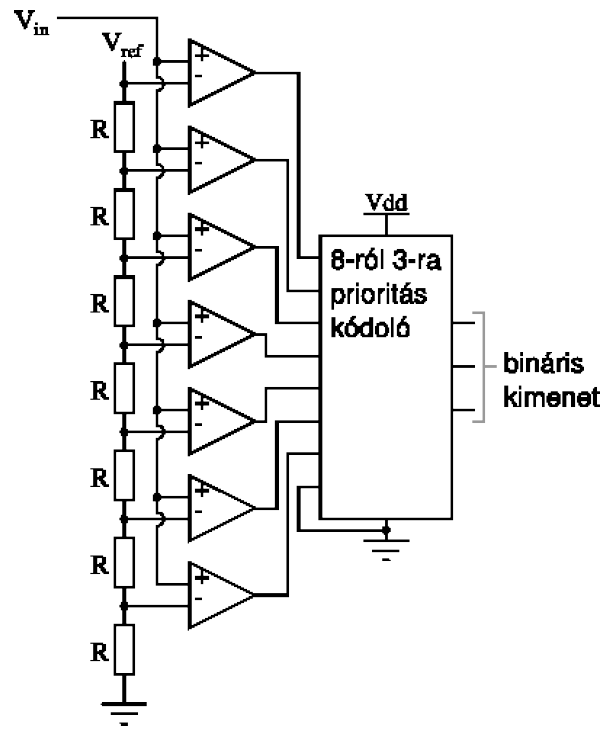
\includegraphics[width=0.5\linewidth]{media/ADC_flash}
	\caption{3 bites párhuzamos (flash) A/D konverter vázlata.}
	\label{fig:adcflash}
\end{figure}

\Aref{fig:adcflash}. ábrán egy $n=3$ bites szimultán ADC áramkört láthatunk. A megvalósításához a digitális szintek számánál 1-gyel kevesebb, azaz jelen esetben $2^n - 1 = 7$ db azonos ellenállásra van szükség, amelyek sorosan kapcsolva egyenlően osztják a referenciafeszültséget. Így az egyes ellenállások közti csomópontokban (a földhöz képest) a digitális szinteknek megfelelő feszültségek állnak elő. A bemenő $V_{in}$ analóg jelet komparátorok sorozata hasonlítja össze az ellenálláslánc $V_{ref}$-ből osztott referenciafeszültségeivel. Amennyiben a komparátor pozitív bemenetére kötött bemenő jel nagyobb a negatívra kötött referenciafeszültségnél, a kimenet logikai 1, ellenkező esetben 0. A komparátorok kimenetét egy kódoló áramkör alakítja át bináris jellé. A kimeneten végeredményül a legmagasabb logikai 1-et tartalmazó bemenet bináris címét kapjuk, azaz a bemenő feszültséget bináris értékké konvertálva. A kódoló áramkör felépíthető kizáró-vagy kapuk és diódás logika felhasználásával, ennek technikai részleteire itt nem térünk ki. A flash konverter a leggyorsabb ADC, mivel az átalakítás egy órajel alatt megtörténik, sok egyéb típustól eltérően (lásd később). További érdekes tulajdonsága a flash konverternek, hogy a digitalizálási szintek csak az ellenálláslánctól függenek, azaz igény esetén nemlineáris skálát is lehet alkalmazni az analóg-digitális átalakításnál az ellenállások megváltoztatásával.



\subsection{Számláló A/D konverter}

\begin{figure}[]
	\centering
	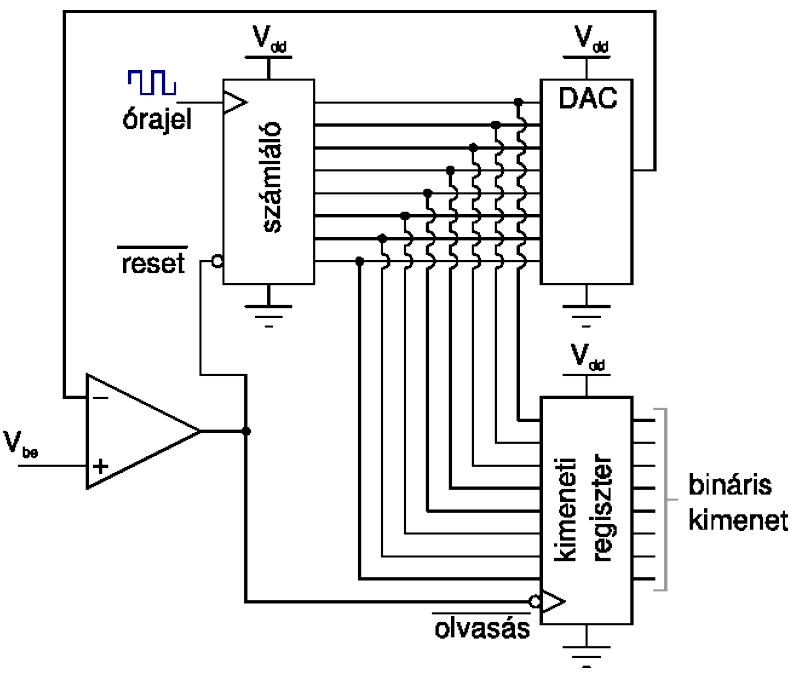
\includegraphics[width=0.7\linewidth]{media/ADC_szamlalo}
	\caption{8 bites számláló A/D konverter vázlata.}
	\label{fig:adcszamlalo}
\end{figure}

A számláló A/D konverter az egyik legegyszerűbb átalakító, vázlatát \aref{fig:adcszamlalo}. ábra mutatja. A berendezés "lelke" egy órajellel vezérelt bináris impulzusszámláló. Ennek kimenetét minden órajelkor egy D/A (!) konverterre vezetjük, ami egy nagy pontosságú $V_{ref}$ feszültségforrásból a számláló értékével arányos analóg feszültséget állít elő. Ezt egy komparátor segítségével összehasonlítjuk a bemenő, mérni kívánt ismeretlen $V_{be}$ analóg jellel. Amikor a DAC kimenő feszültsége eléri a $V_{be}$ feszültséget, akkor a komparátor átbillen, és ez egyrészt beírja a számláló értékét a kimeneti regiszterbe (pl. D tárolókból építhetünk ilyet), másrészt nullázza a számlálót. A mérés során tehát a mérendő értékkel arányos számú impulzus kerül a számlálóba, a mért érték digitális formában rendelkezésre áll. 
A konverter nagy hibája, hogy a mérési (átalakítási) idő függ a mérendő feszültségtől (lásd: \ref{fig:adcszamlalojel}. ábra). Ez az ingadozás a számítógépes jelfeldolgozást (pl. teljesítményspektrum meghatározása) bonyolítja, a digitális szűrést pedig megakadályozza. Gyorsan változó jelek mérésére nem alkalmas.


\begin{figure}[H]
	\centering
	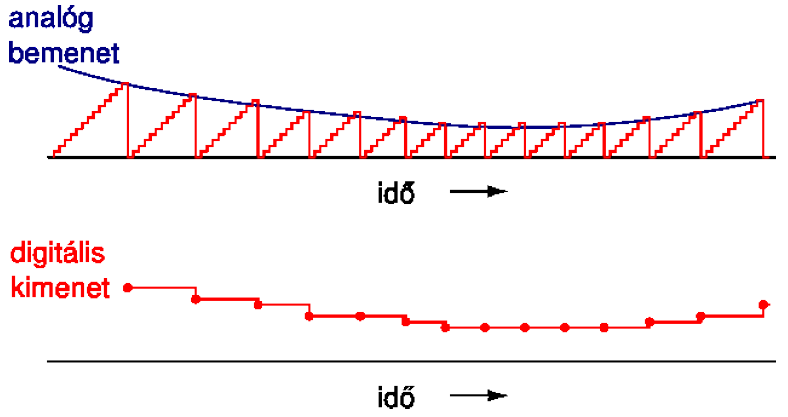
\includegraphics[width=0.7\linewidth]{media/ADC_szamlalo_jel}
	\caption{Számláló A/D konverterrel végzett konverzió szemléltetése. Jól látható a diszkrét lépések számának és az átalakítandó analóg feszültség nagyságának viszonya, illetve a konverzió közti időlépések különbözősége.}
	\label{fig:adcszamlalojel}
\end{figure}


\subsection{Szukcesszív approximációs A/D konverter}

\begin{figure}[]
	\centering
	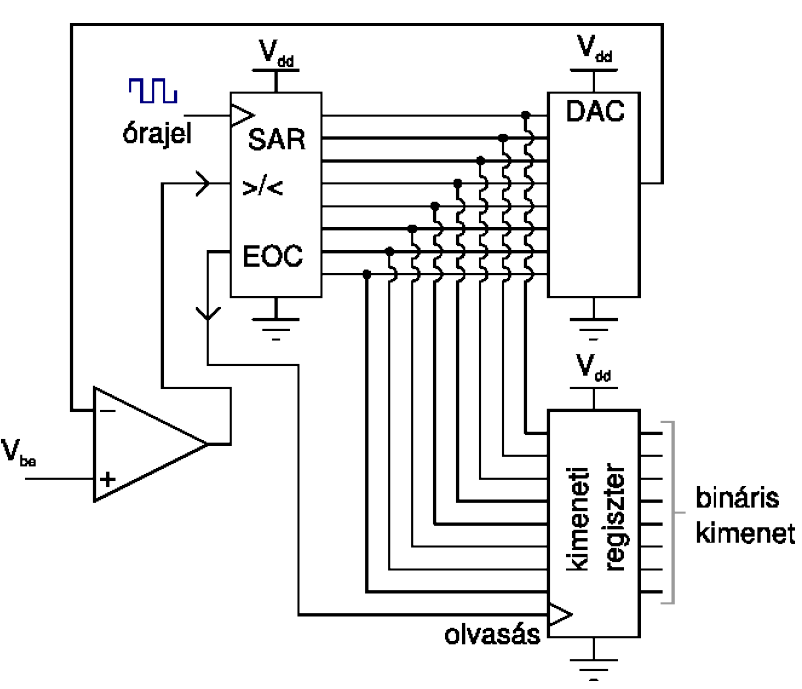
\includegraphics[width=0.7\linewidth]{media/ADC_SAR}
	\caption{8 bites szukcesszív approximációs A/D konverter vázlata.}
	\label{fig:adcsar}
\end{figure}


A szukcesszív approximációs konverter felépítésében és működésében hasonló a számláló A/D konverterhez, azonban annál összetettebb és hatékonyabb. A konverziót egy központi vezérlőlogika irányítja. A számláló helyett szukcesszív approximációs regiszter (SAR) található az áramkörben. A konverzió első lépéseként a SAR legnagyobb helyiértékű bitje (MSB, \textit{most significant bit}) logikai 1-be billen, míg az összes többi 0 marad. Ebből a számláló A/D átalakítóban is látott DAC egység analóg jelet állít elő, ami épp a mérési tartomány ($V_{ref}$) fele. Ezzel a referenciajellel hasonlítja össze a $V_{be}$ mérendő analóg jelet a komparátor. Amennyiben MSB-nél nagyobbnak bizonyul a konvertálandó analóg jel\footnote{Az MSB rövidítés egyaránt utalhat szó szerint egy bináris szám legnagyobb helyiértékű bitjére, annak decimális értékére, illetve az ennek megfelelő nagyságú analóggá konvertált feszültségre.}, a bit értéke 1 marad, ellenkező esetben a vezérlő SAR törli a bitet. Ezáltal kiderül, hogy a mérési tartománynak melyik felébe esik a mérendő jel. 
A további órajelek során a SAR a bináris számrendszer csökkenő helyértékeinek megfelelő biteknél megismétli az előbbi eljárást, miközben a korábban beállított nagyobb helyiértékű bitek változatlanok maradnak. Egy ciklusban tehát mindig feleződik az előző lépésben vizsgált mérési tartomány. A komparátor megvizsgálja, hogy a mérendő mennyiség kisebb vagy nagyobb-e, mint az aktuális mérési tartomány fele: a bit értéke ennek megfelelően áll be. A legkisebb helyiértékű bit (LSB, \textit{least significant bit}) meghatározása után a SAR a bemenő analóg jel digitális értékét tartalmazza (a konverzió pontossága LSB).\footnote{Tekintsünk egy konkrét példát: 13.7~V analóg jel esetén egy 5 bites konverternél $MSB=16$, ez tehát 0-nak adódik. A 32~V-ig terjedő mérési tartománynak mostantól az alsó felét vizsgáljuk. A következő helyiérték már 1, mivel $13.7>8$, tehát 8 és 16 közé szűkült a vizsgálandó tartomány. Így tovább, mivel $8+4<13.7$, $8+4+2>13.7$, $8+4+1<13.7$, a bitek értéke sorban, azaz a bináris szám: 01101. A mérés értéke 13~V-nak adódik, a tizedesjegy csonkolódik, mivel $13.7<14$. 0.7~V a konverziós hiba.}
A konverzió végét az áramkör jelzi (EOC, \textit{end of conversion}), és a kimeneti regiszter ekkor olvassa be a SAR bitjeit. A következő átalakítást a külső áramkör a SAR törlésével indítja.
Figyelemre méltó, hogy a mérési idő a SAR regiszter méretétől, azaz a konverter felbontásától függ, mivel az összehasonlítások száma megegyezik a AD bitjeinek számával (pl. 8 bit esetén 8 ciklus kell a teljes méréshez); a számláló A/D konverterrel ellentétben a konverziós idő a mérendő jel értékétől független. Megemlítendő még, hogy a szukcesszív approximációs ADC működtetéséhez szükség van gyors mintavevő és jelnyújtó (\textit{sample and hold}) áramköri egységekre annak érdekében, hogy a szukcesszív approximáció több órajeles időtartama alatt stabil legyen a konvertált mennyiség. Összességében a szukcesszív approximációs A/D konverter az egyik legelterjedtebb átalakító a számítógépes mérésadatgyűjtő berendezésekben, viszonylag egyszerű felépítése, pontossága és a legtöbb gyakorlati alkalmazáshoz kellőképpen gyors sebessége miatt.



\section{Mintavételi törvény}

A Nyquist-Shannon-törvény kimondja, hogy egy $f_B$ frekvenciájú
tisztán szinuszos jel digitális reprezentációjához legalább $2 \cdot f_B$ frekvenciával szükséges mintavételezést végezni. Mivel az analóg jelek általában nem mentesek a mintavételezési frekvenciánál nagyobb frekvenciájú komponensektől (felharmonikusok), ezért az A/D konverterek bemenetét aluláteresztő szűrőn keresztül kell meghajtani. Ha ezt nem tennénk meg, akkor a mintavételezett jel jelentősen torzulna.



\section{Kvantálási zaj}



\section{$\Delta$-moduláció és $\Delta$-$\Sigma$-moduláció}

\subsection{Tömörítés}


\section{Digitális számábrázolás és műveletvégzés}


%\begin{figure}[H]
%    \begin{center}
%    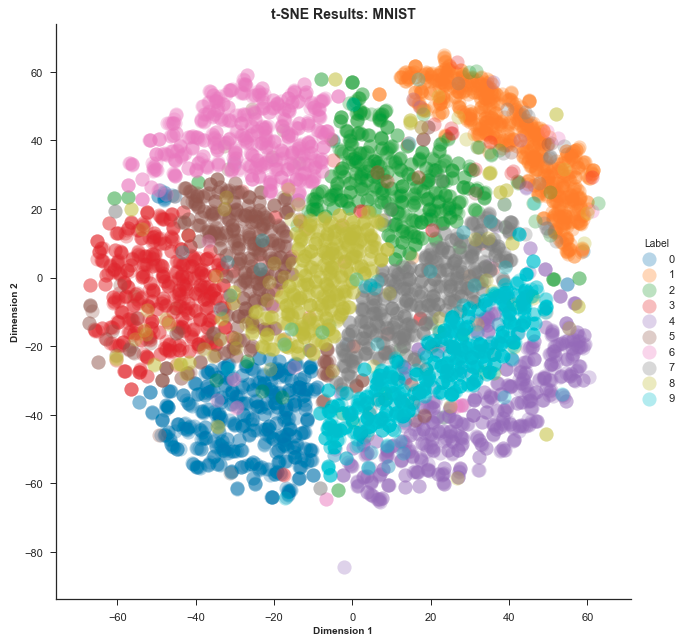
\includegraphics[width=0.5\textwidth]{media/tsneplot.png}
%    \caption{t-SNE plot for MNIST dataset \cite{tsne-article}} 
%    \label{fig:tsneplot}
%    \end{center}
%\end{figure}

\bibliographystyle{plain}
\bibliography{references}

\end{document}
